%!TEX root = main-doc.tex
%
% File: background.tex
%
% Date: ? 
%
% Description:
%   The background is given to ...
%
%
\chapter{Background} \label{chap:background}
\vspace{-1cm}
%\summary{This chapter provides a background on data warehousing and OLAP, extendible multidimensional dense arrays and multidimensional sparse arrays.}

%%%%%%%%%%%%%%%%%%%%%%%%%%%%%%%%%%%%%%%%%%%%%%%%%%%%%%%%%%%%%%%%%%%%%%%%%%%%%%%%
\section{Big Data Representations}
In order to understand data warehouses one also needs to look at ``Big Data''. Big Data can be characterized in the following ways. Big Data has big volume. When it is stored it needs to be scalable by increasing the storage allowing for the data to grow. Big Data has high velocity. Big Data databases need to cope with high speeds, ensuring that the rate at which data comes in is catered for. Big Data has a wide variety of data types. Data comes in any different formats, a clear example of databases that need to cater for variety are multimedia databases for geographic location. These databases need to ensure that spacial data, moving data, structured data, unstructured data and legal documents are captured. Big Data needs to be valid. Data is only useful if it is accurate and reliable. In order to ensure that data is veracity one must ensure that the data is stored correctly and not manipulated accidentally. Big Data has big value. As discussed in Chapter \ref{chap:introduction} data is a crucial component in improving intelligent business decisions.

There are several universal formats for representing Big Data including Hierarchical Data Format (HDF5), Network Common Data Form (NetCDF), Flexible Image Transport System (FITS), NumPy, PyTable, TileDB. Platforms for data analysis include Hadoop, Weka, RapidMiner, Pentaho, Scikit-learn, Apache Spark and R \cite{tiledb:tm101}.

%%%%%%%%%%%%%%%%%%%%%%%%%%%%%%%%%%%%%%%%%%%%%%%%%%%%%%%%%%%%%%%%%%%%%%%%%%%%%%%%
\section{Data Warehousing}
In Chapter \ref{chap:introduction} we mentioned how important information is in the current world \cite{golfarelli:2009:dwd}. It was also discussed that due to the vast amounts of data being created and stored every day and the inability for traditional database methods (e.g. SQL database systems) to deal with such large volumes of data, data warehousing was created for decision making.

Bill Inmon defines data warehousing as an architecture that is a subject-oriented, non-volatile, integrated, time variant collection of data created for the purpose of management’s decision making. Ralph Kimball defines a data warehouse as a copy of transaction data specifically structured for query and analysis.

The modern advanced data warehousing processes allow for OLAP by creating a new data repository that integrates basic data from various sources, arranges the data formats and makes the data available for analysis and decision-making \cite{golfarelli:2009:dwd}. OLAP queries require dynamic, multidimensional analyses of huge quantities of data to process records for decision-making. OLAP queries make use of multidimensional representations of data warehouses as the data is viewed as points in space whose dimensions correspond to many possible analysis dimensions \cite{golfarelli:2009:dwd}. A 3D data warehouse cube is given in Figure \ref{fig:exampleCube} to explicitly show why multidimensional representations are important for OLAP.

 \begin{figure}[H]
	\centering
	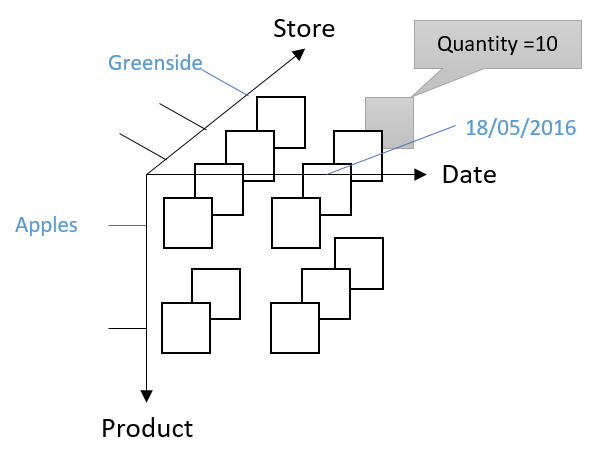
\includegraphics[width=0.6\linewidth]{exampleCube2}
	\caption{An Example of a Multidimensional Data Warehouse}
	\label{fig:exampleCube}
\end{figure}

The data warehousing and OLAP operations that are most commonly used include: Get, Insert, Addition, Multiplication, Subtraction, Division, roll-up, drill-down, slice-and-dice, pivot, drill-across, drill-through, and range or box access. We will show how these operations are executed in our XSAS representation.

%%%%%%%%%%%%%%%%%%%%%%%%%%%%%%%%%%%%%%%%%%%%%%%%%%%%%%%%%%%%%%%%%%%%%%%%%%%%%%%%
\section{Methodologies}
In order to develop a model for extendible multi-dimensional sparse arrays, the current representations of extendible multi-dimensional arrays must be analysed. The study of the current representations will give a clear indication of how to integrate the representation of extendible multi-dimensional sparse arrays, so that the model can easily be integrated into the current system, preventing unnecessary additional costs. Once a model has been developed, compression of data as well as computing speed will be assessed.

%%%%%%%%%%%%%%%%%%%%%%%%%%%%%%%%%%%%%%%%%%%%%%%%%%%%%%%%%%%%%%%%%%%%%%%%%%%%%%%%
\section{Sparse Array Representations}
There are numerous studies that have been conducted on the efficiency of different sparse array representation schemes \cite{wang:2014sar,goil:bess}. In order to accurately understand these models, we must first understand exactly what is meant by a sparse array. If an array is sparse, it has very few non-zero elements relative to the product of the cardinalities \cite{wang:2014sar}.

There are three main methods used for 2-dimensional sparse array representations, namely: 
\begin{compactenum}
	\item Matrix Market (known as a relational table or a Triplicate)
	\item Linked list
	\item Compressed Row (or alternatively Column) Storage (CRS/CCS)
\end{compactenum}	

These three methods are discussed in more detail in Chapter \ref{chap:methodology}.

There are six other methods that are used for multidimensional representations, namely: 
\begin{compactenum}
	\item Bit-Encoded Sparse Storage (BESS) 
	\item Extended CRS/CCS known as xCRS and xCCS
	\item PATRICIA Trie Compressed Storage (PTCS)
	\item Bit-Encoded Compressed Row (or Column) storage (BxCRS/BxCCS)
	\item Hybrid approach (Hybrid) that combines BESS with xCRS
\end{compactenum}

BESS is the simplest low level storage scheme that chops every point into bit block dimensions. BESS has decent storage, but is traditionally static with the maximum number of chunks being determined algorithmically.

The PTCS is unique and allows for extendibility with regards to data warehousing operations. BESS and PTCS are discussed further in Chapter \ref{chap:methodology}.

%%%%%%%%%%%%%%%%%%%%%%%%%%%%%%%%%%%%%%%%%%%%%%%%%%%%%%%%%%%%%%%%%%%%%%%%%%%%%%%%
%\section{Dynamic Sparse Arrays}
%Increasing Density
%\begin{itemize}
%	\item Bounds and structure remain the same
%	\item new elements are slot into a chunk where there was a free space
%\end{itemize}
%Increasing Bound

%%%%%%%%%%%%%%%%%%%%%%%%%%%%%%%%%%%%%%%%%%%%%%%%%%%%%%%%%%%%%%%%%%%%%%%%%%%%%%%%
\section{Impact}

%%%%%%%%%%%%%%%%%%%%%%%%%%%%%%%%%%%%%%%%%%%%%%%%%%%%%%%%%%%%%%%%%%%%%%%%%%%%%%%%
\section{New Results}
